\begin{figure}[htbp]
\section*{ LMNA (Part 1 of 2)}
\centering
\begin{subfigure}[b]{0.95\textwidth}
\centering
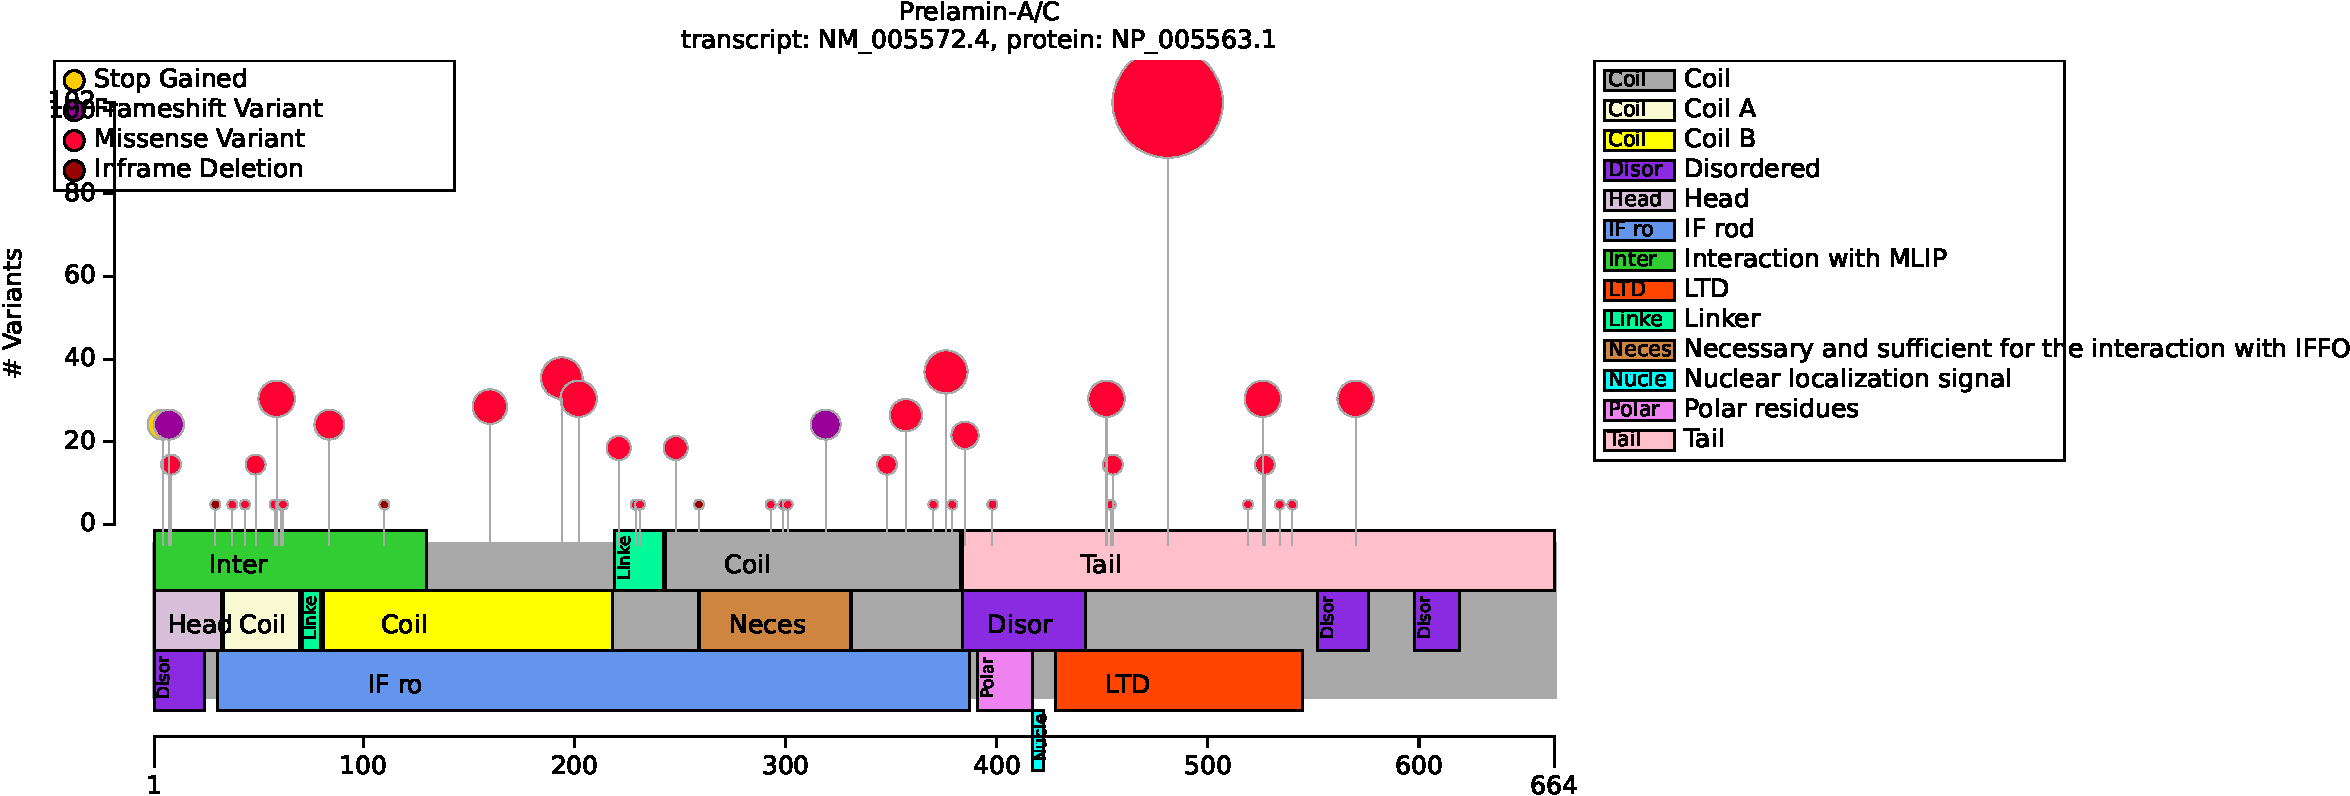
\includegraphics[width=\textwidth]{ img/LMNA_protein_diagram.pdf} 
\captionsetup{justification=raggedright,singlelinecheck=false}
\caption{Distribution of variants in LMNA}
\end{subfigure}

\vspace{2em}

\begin{subfigure}[b]{0.95\textwidth}
\centering
\resizebox{\textwidth}{!}{
\begin{tabular}{llllrr}
\toprule
HPO term & missense & other & p-value & adj. p-value\\
\midrule
Loss of truncal subcutaneous adipose tissue [HP:0009002] & 104/104 (100\%) & 4/11 (36\%) & $7.53\times 10^{-9}$ & $1.28\times 10^{-7}$\\
Elevated hemoglobin A1c [HP:0040217] & 73/101 (72\%) & 6/24 (25\%) & $3.11\times 10^{-5}$ & $2.64\times 10^{-4}$\\
\bottomrule
\end{tabular}
}
\captionsetup{justification=raggedright,singlelinecheck=false}
\caption{Fisher Exact Test performed to compare HPO annotation frequency with respect to missense and other. Total of
        17 tests were performed. }
\end{subfigure}
\vspace{2em}
\begin{subfigure}[b]{0.95\textwidth}
\centering
\resizebox{\textwidth}{!}{
\begin{tabular}{llllrr}
\toprule
HPO term & NLS Upstream & other & p-value & adj. p-value\\
\midrule
Lipodystrophy [HP:0009125] & 10/93 (11\%) & 132/158 (84\%) & $1.73\times 10^{-31}$ & $3.81\times 10^{-30}$\\
Pancreatitis [HP:0001733] & 4/7 (57\%) & 14/110 (13\%) & 0.011 & 0.023\\
Dilated cardiomyopathy [HP:0001644] & 35/70 (50\%) & 5/102 (5\%) & $4.20\times 10^{-12}$ & $4.62\times 10^{-11}$\\
Atrioventricular block [HP:0001678] & 17/36 (47\%) & 8/116 (7\%) & $2.11\times 10^{-7}$ & $1.54\times 10^{-6}$\\
Achilles tendon contracture [HP:0001771] & 21/85 (25\%) & 19/30 (63\%) & $2.66\times 10^{-4}$ & $6.51\times 10^{-4}$\\
Foot joint contracture [HP:0008366] & 21/81 (26\%) & 19/27 (70\%) & $6.20\times 10^{-5}$ & $3.41\times 10^{-4}$\\
Lower-limb joint contracture [HP:0005750] & 22/82 (27\%) & 19/27 (70\%) & $8.20\times 10^{-5}$ & $3.61\times 10^{-4}$\\
Limb joint contracture [HP:0003121] & 23/83 (28\%) & 19/27 (70\%) & $1.71\times 10^{-4}$ & $4.71\times 10^{-4}$\\
Elbow contracture [HP:0034391] & 21/83 (25\%) & 18/26 (69\%) & $1.04\times 10^{-4}$ & $3.81\times 10^{-4}$\\
Upper-limb joint contracture [HP:0100360] & 21/81 (26\%) & 18/26 (69\%) & $1.23\times 10^{-4}$ & $3.86\times 10^{-4}$\\
\bottomrule
\end{tabular}
}
\captionsetup{justification=raggedright,singlelinecheck=false}
\caption{Fisher Exact Test: HPO annotation frequency and NLS Upstream vs other variants.  22 tests were performed in total. }
\end{subfigure}
\caption{See following page for caption}
\end{figure}


\begin{figure}[htbp]
        \section*{ LMNA (Part 2 of 2)}
\vspace{2em}
\begin{subfigure}[b]{0.95\textwidth}
\centering
\resizebox{\textwidth}{!}{
\begin{tabular}{llllrr}
\toprule
HPO term & NLS Upstream & other & p-value & adj. p-value\\
\midrule
Lipodystrophy [HP:0009125] & 9/88 (10\%) & 133/163 (82\%) & $1.72\times 10^{-29}$ & $4.12\times 10^{-28}$\\
Dilated cardiomyopathy [HP:0001644] & 35/69 (51\%) & 5/103 (5\%) & $2.20\times 10^{-12}$ & $2.64\times 10^{-11}$\\
Atrioventricular block [HP:0001678] & 17/35 (49\%) & 8/117 (7\%) & $1.19\times 10^{-7}$ & $9.50\times 10^{-7}$\\
Achilles tendon contracture [HP:0001771] & 17/81 (21\%) & 23/34 (68\%) & $3.37\times 10^{-6}$ & $8.99\times 10^{-6}$\\
Foot joint contracture [HP:0008366] & 17/77 (22\%) & 23/31 (74\%) & $6.70\times 10^{-7}$ & $4.02\times 10^{-6}$\\
Lower-limb joint contracture [HP:0005750] & 18/78 (23\%) & 23/31 (74\%) & $1.55\times 10^{-6}$ & $5.32\times 10^{-6}$\\
Limb joint contracture [HP:0003121] & 19/79 (24\%) & 23/31 (74\%) & $2.06\times 10^{-6}$ & $6.18\times 10^{-6}$\\
Elbow contracture [HP:0034391] & 17/79 (22\%) & 22/30 (73\%) & $9.63\times 10^{-7}$ & $4.62\times 10^{-6}$\\
Upper-limb joint contracture [HP:0100360] & 17/77 (22\%) & 22/30 (73\%) & $1.36\times 10^{-6}$ & $5.32\times 10^{-6}$\\
\bottomrule
\end{tabular}
}
\captionsetup{justification=raggedright,singlelinecheck=false}
\caption{Fisher Exact Test performed to compare HPO annotation frequency with respect to NLS Upstream and other. Total of
        24 tests were performed. }
\end{subfigure}
\vspace{2em}
\begin{subfigure}[b]{0.95\textwidth}
\centering
\resizebox{\textwidth}{!}{
\begin{tabular}{llllrr}
\toprule
HPO term & A & B & p-value & adj. p-value\\
\midrule
Lipodystrophy [HP:0009125] & 15/15 (100\%) & 127/236 (54\%) & $1.87\times 10^{-4}$ & $3.11\times 10^{-4}$\\
Elevated hemoglobin A1c [HP:0040217] & 0/15 (0\%) & 79/110 (72\%) & $5.65\times 10^{-8}$ & $2.82\times 10^{-7}$\\
Muscle weakness [HP:0001324] & 0/15 (0\%) & 63/124 (51\%) & $6.07\times 10^{-5}$ & $1.52\times 10^{-4}$\\
Proximal muscle weakness [HP:0003701] & 0/15 (0\%) & 53/114 (46\%) & $3.63\times 10^{-4}$ & $4.54\times 10^{-4}$\\
\bottomrule
\end{tabular}
}
\captionsetup{justification=raggedright,singlelinecheck=false}
\caption{         Fisher Exact Test performed to compare HPO annotation frequency with respect to A and B. Total of
        5 tests were performed. }
\end{subfigure}
\vspace{2em}
\begin{subfigure}[b]{0.95\textwidth}
\captionsetup{justification=raggedright,singlelinecheck=false}
\resizebox{\textwidth}{!}{
\begin{tabular}{llllrr}
\toprule
Description & Variable & Genotype (A) & Genotype (B) & p-value & xrefs\\
\midrule
Assign a phenotype score that is equivalent to the count of present phenotypes that are either an exact match to the query terms or their descendants & HPO group count & NLS Upstream & other & $1.83\times 10^{-16}$ & -\\
\bottomrule
\end{tabular}
}
\caption{ HPO Group Count to compare NLS Upstream and other with respect to HPO group count. }
\end{subfigure}

\vspace{2em}

\caption{ The cohort comprised 266 individuals (150 females, 99 males, 17 with unknown sex). 11 of these individuals were reported to be deceased. 
A total of 152 HPO terms were used to annotate the cohort. Disease diagnoses: Lipodystrophy, familial partial, type 2 (OMIM:151660) (127 individuals), 
Cardiomyopathy, dilated, 1A (OMIM:115200) (68 individuals), Emery-Dreifuss muscular dystrophy 2, autosomal dominant (OMIM:181350) (41 individuals), 
Hutchinson-Gilford progeria (OMIM:176670) (15 individuals), LMNA-related congenital muscular dystrophy (OMIM:613205) (15 individuals). 
Numerous LMNA genotype-phenotype correlations have been described. The literature is summarized in \cite{PMID_32413188}. 
Cardiac involvement in multisystem laminopathies prevails with mutations upstream of the nuclear localisation signal \cite{PMID_30402260}.
A total of 266 unique variant alleles were found in \textit{LMNA} (transcript: \texttt{NM\_005572.4}, protein id: \texttt{NP\_005563.1}).}
\end{figure}
